\documentclass[12pt]{report}

\usepackage{setspace}
%\setstretch{2.5} % for custom spacing
\setlength{\parindent}{4em}

\usepackage{fancyvrb}
\usepackage{graphicx}
\usepackage{geometry}

\geometry{letterpaper, portrait, margin=1in}

%%%Title Page%%%
\title{
  Lab 04
\bigbreak BUFFALO Utility Subroutines
}

\author{
{\normalsize
\begin{tabular}{l r}
& \textbf{Zachary Davis}\\
\textbf{Category} & zachdav@uga.edu\\
\hline
Lab Part 1 & Taking In A Character\\
Lab Part 2 & Reporting Voltage\\
Lab Part 3 & Combining The Two\\
\end{tabular}
}
}

\date{\bigskip
\today}
%%%%%%%%%%%%


\begin{document}
\maketitle
\section*{Introduction}
	\paragraph{}
		N/A

\section*{Lab Procedure}
	\paragraph{}
		N/A

\section*{Conclusion}
	\paragraph{}
		N/A

\section*{References}
	\paragraph{}
		N/A

\section*{Part 1}

	\begin{center}
		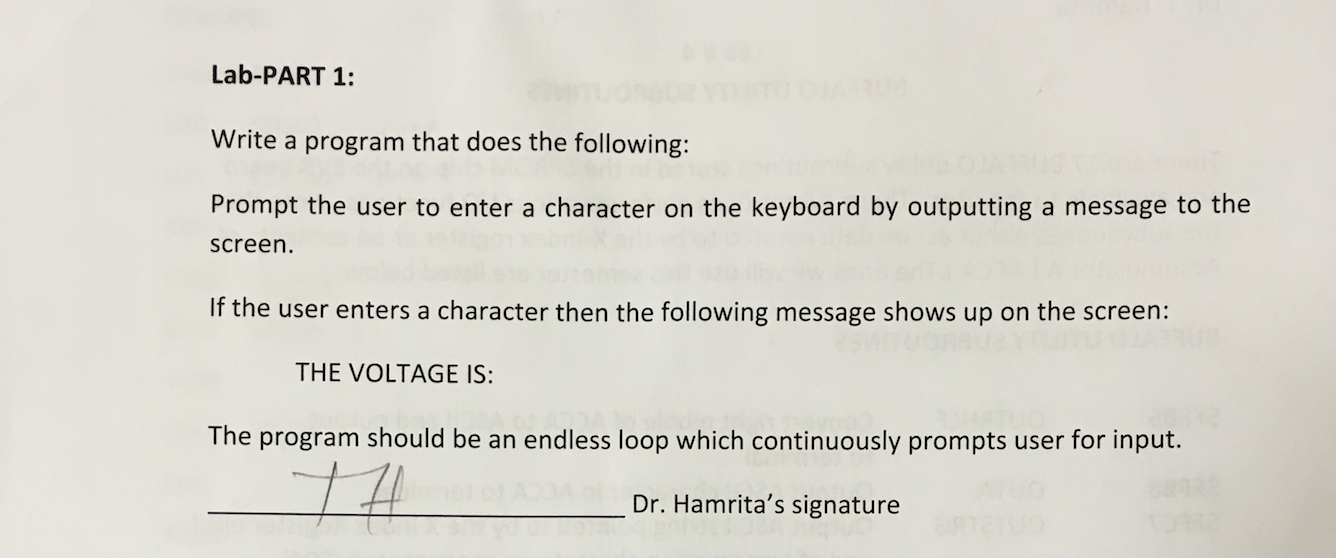
\includegraphics[scale=.70]{p1.PNG}
	\end{center}

\section*{Part 2}

	\begin{center}
		\includegraphics[scale=.155]{p2.PNG}
	\end{center}

\section*{Part 3}

	\begin{center}
		\includegraphics[scale=.155]{p3.PNG}
	\end{center}

\section*{Hardware Schematic}
	\paragraph{}
		N/A

\section*{Pseudo Code For The Software Developed}
	A few equate statements from the BUFFALO utility subroutines to be used
	in the following programs.  The included sunroutines are OUTA (output the
	ASCII character in ACCA), OUTSTRG(O) (Either output the string with or without 
	a carrage return), INCHAR (waits to read in an ASCII character from the 
	terminal and load it into ACCA), OUTRHLF (output the right nibble of ACCA to 
	the terminal), and OUTCRLF (output an ASCII return carriage).\\\\

	EQUATES:\\
	Define four messages for each of the three programs\\
	Message1 is "Enter A Character: "\\
	Message2 is "The Voltage Is: "\\
	Message3 is "."\\
	Message4 is " Volts"\\\\

	VARIBALES:\\
	Define org statement for \$D000 for variable as asked in the lab instructions\\
	Mvolts is a 2 byte Variable\\\\

	MAIN:\\
	Start the program at address \$D002\\
	Jump to the subroutine for the part of the lab the user wishes to use (Part 1-3).\\
	Software interrupt\\
	End the program\\\\

	PART1:\\
	Load accumulator X with the Message1 prompt\\
	Output the string to the terminal\\
	Wait for a character input\\
	Load a response Message2 into accumulator X\\
	Output the string to the terminal\\
	Return to the MAIN\\\\

	PART2:\\
	The program assumes that correct values are stored in address \$DB01-\$DB04\\
	Load accumulator A with the value in \$DB01 and print it without a return carriage\\
	Repeat for the values in \$DB02\\
	Load accumulator X with a decimal point (Message3) and output it without a return carriage\\
	Repeat output for address \$DB03 and \$DB04\\
	Load accumulator X with Message4 and output it with a return carriage\\
	Return to MAIN\\\\

	PART3:\\
	Jump to part1 subroutine\\
	Convert hexidecimal to binary coded decimal with the subroutine from lab 3\\
	Jump to part2 subroutine\\
	Return to MAIN\\\\

	BINBCD:\\
	Load the value of \$D000 and \$D001 into accumulator D\\
	Load accumulator X with the divisor 2710\\
	Divide D with X and store the result into \$DB00\\
	Repeat with a divisor of 3E8\\
	Store the result into \$DB01\\
	Repeat with a divisor of 64\\
	Store the result into \$DB02\\
	Repeat with a divisor of A\\
	Store the result into \$DB03\\
	Store whats left into \$DB04\\
	Return to the subroutine part3\\


\section*{Program Flowchart}
	\begin{center}
		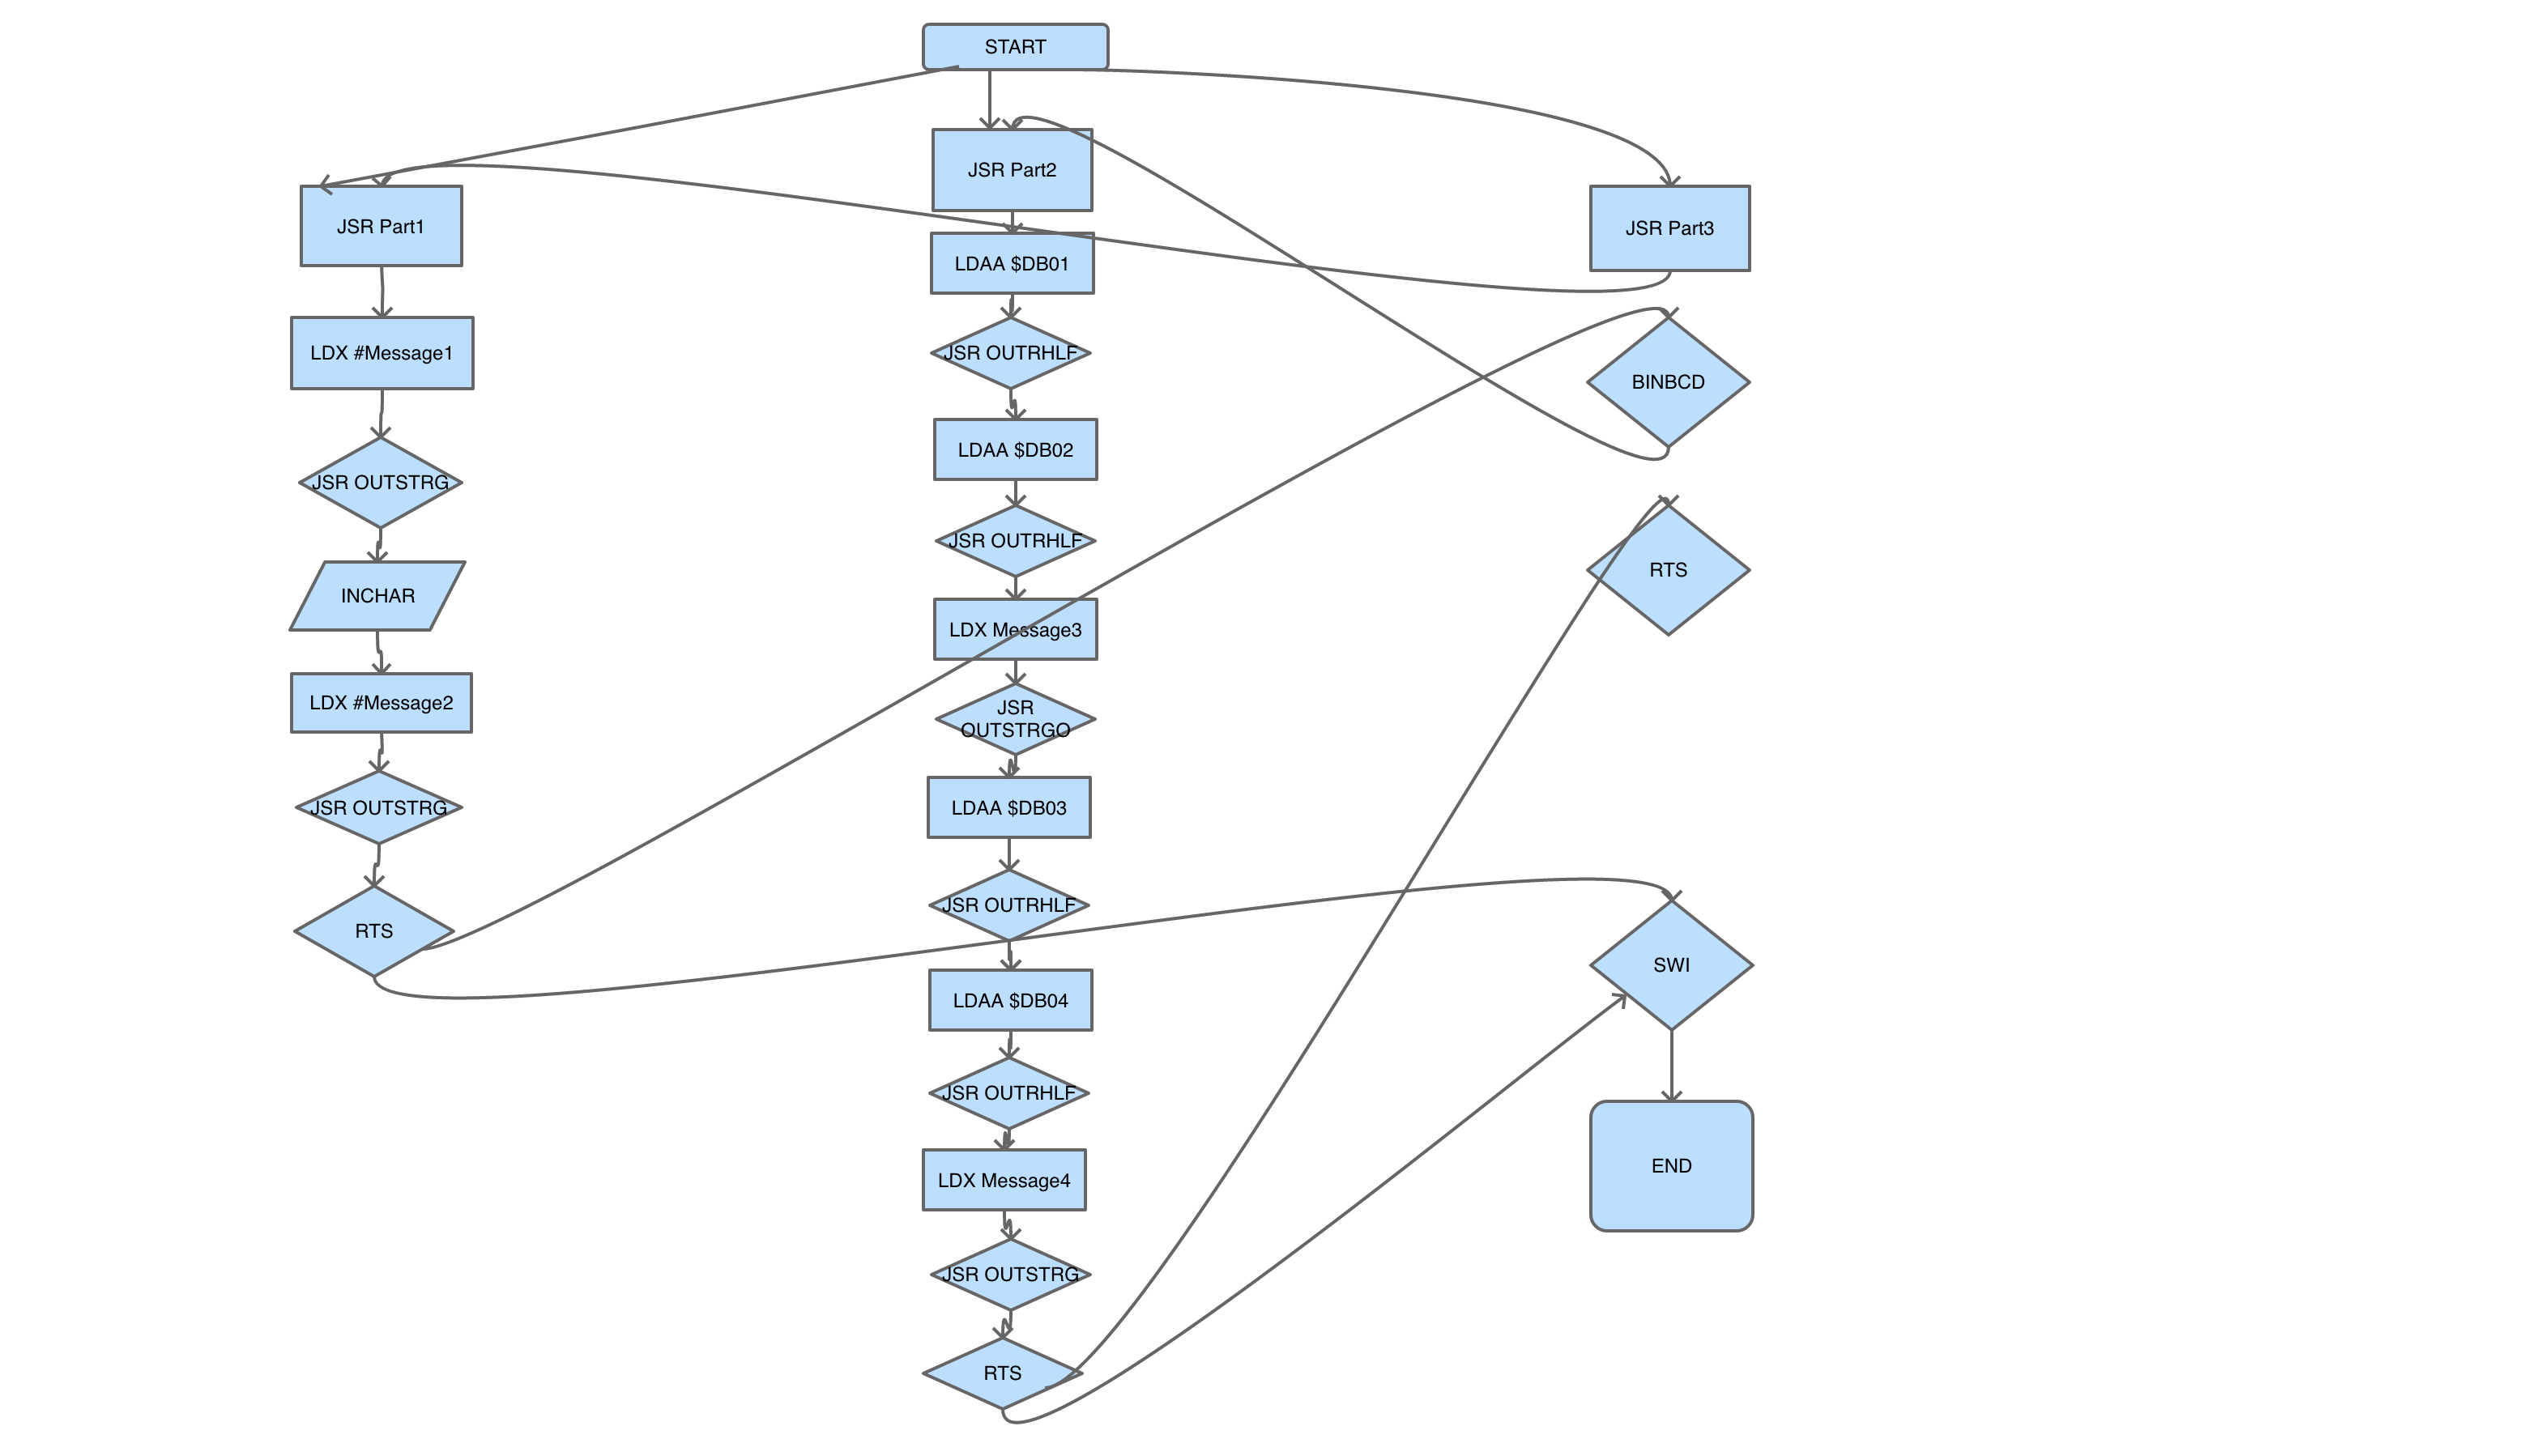
\includegraphics[scale=.18]{flowchart.PNG}
	\end{center}

\section*{Program Listing}
	\begin{Verbatim}[frame=single, fontsize=\small]
********************************************************************************         
         ;Including a few of the BUFFALO utility subroutines for the program.
OUTA     EQU  $FFB8  ;Output the ASCII character in ACCA to the terminal
OUTSTRG  EQU  $FFC7  ;Output the ASCII string pointed to in the X register
OUTSTRGO EQU  $FFCA  ;Same as above without leading return carriage or line feed
OUTRHLF  EQU  $FFB5  ;Ouput the right nibble of ACCA in ASCII to the terminal
OUTCRLF  EQU  $FFC4  ;Output ASCII return carriage and line feed to terminal
INCHAR   EQU  $FFCD  ;Input ASCII character into ACCA and echo it to the terminal
******************************************************************************** 

******************************************************************************** 
         ;Defining useful program messages.
Message1 FCC  "Enter a Character: "
         FCB  $04
Message2 FCC  "The Voltage is: "
         FCB  $04
Message3 FCC  "."
         FCB  $04
Message4 FCC  " Volts."
******************************************************************************** 

******************************************************************************** 
         ;An org statement for the memory of the program.  This reserves two 
         ;bytes of memory for part 3 of the lab.  It is intended for the user
         ;to memory modify (MM) the address of D000 and D001 with a mV in hex.
         ORG  $D000
MVOLTS   RMB  2  ;Reserves 2 memory bytes starting at D000
******************************************************************************** 
         
         ;This is the main of the program.  Each subroutine that follows
         ;is labeled corresponding to each part of the lab.
         ;To test a part of the lab you simply change the label following
         ;jump to subroutine.
         ORG  $D002
Main:    JSR  Part1 ;or Part2 ;or Part3
         SWI        ;Software Interrupt
         END

         ;Prints the string stored in Message1 and waits for the user to
         ;input a character.  It then in responce returns the string in
         ;Message2.  The procedure is in an infinite loop.
Part1:   LDX  #Message1
         JSR  OUTSTRG
         JSR  INCHAR
         LDX  #Message2
         JSR  OUTSTRG
         RTS

         ;Print the right nibble of DB01 and DB02, then print the "." string,
         ;then the right nibble of DB03 and DB04, followed finally by the
         ;string " Volts."
Part2:   LDAA $DB01
         JSR  OUTRHLF
         LDAA $DB02
         JSR  OUTRHLF
         LDX  #Message3
         JSR  OUTSTRGO
         LDAA $DB03
         JSR  OUTRHLF
         LDAA $DB04
         JSR  OUTRHLF
         LDX  #Message4
         JSR  OUTSTRGO
         JSR  OUTCRLF
         RTS
         
         ;This program combines all the parts of the previous labs and parts.
         ;It waits for the user to enter any random character and then converts
         ;the value stored in D000 and D001 from hex to binary coded decimal.
         ;Finally it outputs that BCD to the terminal along with a message.
Part3:   JSR  Part1
         JSR  BINBCD
         JSR  Part2
         RTS

         ;This subroutine takes the values stored in D000 and D001 into 
         ;accumulator D (2 bytes).  Then it converts the value from hex
         ;to binary coded decimal storing each digit in DB00-DB04.
BINBCD   LDD  $D000
         LDX  #$2710  ;Divisor
         IDIV
         XGDX         ;Swap
         STAB $DB00
         XGDX         ;Swap
         LDX  #$3E8   ;Divisor
         IDIV
         XGDX         ;Swap
         STAB $DB01
         XGDX         ;Swap
         LDX  #$64    ;Divisor
         IDIV
         XGDX         ;Swap
         STAB $DB02
         XGDX         ;Swap
         LDX  #$A     ;Divisor
         IDIV
         XGDX         ;Swap
         STAB $DB03
         XGDX         ;Swap
         STAB $DB04
         RTS
	\end{Verbatim}
\end{document}